\documentclass[aspectratio=169, 10pt]{beamer} 
\usepackage{lmodern}

% ==================== PAKIETY ==================== 
\usepackage[utf8]{inputenc} 
\usepackage[T1]{fontenc} 
\usepackage[english]{babel} 
\usepackage{amsmath,amssymb,amsfonts} 
\usepackage{graphicx} 
\graphicspath{{images/}}
\usepackage{xcolor}
\usepackage{fontawesome5}
\usepackage{listings}
\usepackage{etoolbox}
\usepackage{tikz} 
\usetikzlibrary{shapes.symbols, shapes.geometric, arrows.meta, positioning, fit, calc, shadows, decorations.pathreplacing, decorations.pathmorphing, shapes.gates.logic.US} 

% ==================== MOTYW I KOLORY ==================== 
\usetheme{Madrid} 
\useinnertheme{rounded} 
\useoutertheme{miniframes}

% Definiowanie własnej, nowoczesnej palety kolorów 
\definecolor{DeepBlue}{RGB}{20, 45, 85}
\definecolor{AccentOrange}{RGB}{235, 90, 20} 
\definecolor{LightGray}{RGB}{245, 246, 250}
\definecolor{mygreen}{RGB}{0, 153, 37}

% --- KOLORY DLA KODU (VS Code High Contrast) ---
\definecolor{VSDarkBg}{RGB}{25, 25, 25}        
\definecolor{VSText}{RGB}{245, 245, 245}       
\definecolor{VSBlue}{RGB}{80, 180, 255}        
\definecolor{VSPurple}{RGB}{210, 110, 210}     
\definecolor{VSString}{RGB}{255, 140, 80}      
\definecolor{VSComment}{RGB}{80, 220, 80}      

% --- KOLORY PRZYCISKÓW OKNA (macOS) ---
\definecolor{MacRed}{RGB}{255, 95, 86}
\definecolor{MacYellow}{RGB}{255, 189, 46}
\definecolor{MacGreen}{RGB}{39, 201, 63}

% Ustawienia kolorów beamera
\setbeamercolor{palette primary}{bg=DeepBlue, fg=white} 
\setbeamercolor{palette secondary}{bg=DeepBlue!80!black, fg=white} 
\setbeamercolor{palette tertiary}{bg=DeepBlue!90!black, fg=white} 
\setbeamercolor{title}{bg=DeepBlue, fg=white} 
\setbeamercolor{frametitle}{bg=DeepBlue, fg=white} 
\setbeamercolor{structure}{fg=DeepBlue} 
\setbeamercolor{item}{fg=AccentOrange} 
\setbeamercolor{alerted text}{fg=AccentOrange} 
\setbeamercolor{block title}{bg=DeepBlue, fg=white} 
\setbeamercolor{block body}{bg=LightGray, fg=black} 
\setbeamercolor{block title example}{bg=AccentOrange, fg=white} 
\setbeamercolor{block body example}{bg=AccentOrange!10, fg=black}
\setbeamercolor{vscodelisting}{bg=VSDarkBg} % Tło dla bloków kodu

% Płaskie, nowoczesne cienie pod blokami 
\setbeamertemplate{blocks}[rounded][shadow=true]
\setbeamertemplate{navigation symbols}{}

% ==================== FORMATOWANIE KODU (LISTINGS) ==================== 
\lstset{ 
    language=Python, 
    basicstyle=\color{VSText}\ttfamily\footnotesize, 
    keywordstyle=\color{VSBlue}\bfseries, 
    stringstyle=\color{VSString}, 
    commentstyle=\color{VSComment}\itshape, 
    deletekeywords={import, from, as, return, if, elif, else, for, while, in, and, or, not, True, False},
    classoffset=1,
    morekeywords={import, from, as, return, if, elif, else, for, while, in, and, or, not, True, False},
    keywordstyle=\color{VSPurple}\bfseries,
    classoffset=0, 
    numbers=left, 
    numberstyle=\tiny\color{gray}, 
    stepnumber=1, 
    breaklines=true, 
    showstringspaces=false,
    xleftmargin=15pt,
    xrightmargin=5pt,
    backgroundcolor=, 
    frame=none 
}

% Automatyczne owijanie kodu w tło z przyciskami w stylu okna macOS!
\BeforeBeginEnvironment{lstlisting}{%
    \begin{beamercolorbox}[rounded=true, sep=2mm, wd=\linewidth]{vscodelisting}%
    % Rysowanie przycisków okna
    
\begin{tikzpicture}
        \fill[MacRed] (0,0) circle (3pt);
        \fill[MacYellow] (0.35,0) circle (3pt);
        \fill[MacGreen] (0.70,0) circle (3pt);
    \end{tikzpicture}%
    \vspace{-0.2cm}% Lekkie podniesienie kodu, by ładnie przylegał do "paska tytułowego"
}
\AfterEndEnvironment{lstlisting}{\end{beamercolorbox}}
% ==================== DANE PREZENTACJI ==================== 
\title[FHE - Part III]{\textbf{Fully Homomorphic Encryption (FHE)}\\ \Large Part III: Practical Introduction to OpenFHE (Python)}
\author{Ksawery Możdżyński}
\date{}

\begin{document}

% Title slide
\begin{frame}
\titlepage
\end{frame}

% ==========================================
% AGENDA
% ==========================================
\begin{frame}{Agenda for Today}
\Large
\begin{itemize}
    \item[\textcolor{AccentOrange}{\faPython}] \textbf{1. Introduction to OpenFHE} \\
    \textcolor{gray}{\small Architecture, openfhe-python wrapper, and setup}
    \vspace{0.3cm}

    \item[\textcolor{AccentOrange}{\faMicrochip}] \textbf{2. FHEW Scheme: Boolean Logic} \\
    \textcolor{gray}{\small Gate evaluation, fast bootstrapping, and the "Mystery Circuit"}
    \vspace{0.3cm}

    \item[\textcolor{AccentOrange}{\faCalculator}] \textbf{3. BGV Scheme: Exact Arithmetic} \\
    \textcolor{gray}{\small Integer operations, SIMD batching, and evaluation keys}
    \vspace{0.3cm}
    
    \item[\textcolor{AccentOrange}{\faBrain}] \textbf{5. CKKS Scheme} \\
    \textcolor{gray}{\small Introduction to approximate real-number arithmetic}
\end{itemize}
\end{frame}
\section{Introduction}

% --- SLAJD 1: Co to jest OpenFHE? ---
\begin{frame}{What is OpenFHE?}
\begin{columns}[T]
% Lewa kolumna z tekstem
\begin{column}{0.48\textwidth}
    \vspace{0.2cm}
    \begin{itemize}
        \item \textbf{OpenFHE} is a powerful, open-source FHE library written in C++.
        \item It provides a \textbf{unified API} for all major cryptographic FHE schemes.
        \vspace{0.8cm}
        \item \textbf{Why openfhe-python?} 
        \item It acts as a user-friendly wrapper. You write code in Python, but the computations run at the raw execution speed of the underlying C++ engine!
    \end{itemize}
\end{column}

% Prawa kolumna z grafiką (Stos technologiczny)
\begin{column}{0.48\textwidth}
    \centering
    \vspace{0.2cm}
    % Zmniejszone skalowanie i ciaśniejszy układ zapobiegną ucinaniu obrazka
    \resizebox{0.85\textwidth}{!}{
    \begin{tikzpicture}[
        >=stealth,
        layer/.style={draw=DeepBlue, thick, rectangle, minimum width=4.5cm, minimum height=1.0cm, align=center, rounded corners, font=\large\bfseries, drop shadow},
        arrow/.style={->, ultra thick, AccentOrange}
    ]
    
    % Warstwa 1: Python
    \node[layer, fill=LightGray, text=DeepBlue] (python) {\faPython \ Your Python Script};
    
    % Warstwa 2: Wrapper 
    \node[layer, fill=AccentOrange!20, draw=AccentOrange, text=black, below=0.5cm of python] (wrapper) {\faBox \ openfhe-python \\ \normalsize (API Wrapper)};
    
    % Warstwa 3: C++ Core
    \node[layer, fill=DeepBlue, text=white, below=0.5cm of wrapper] (cpp) {\faCogs \ openFHE};
    
    % Strzałki przepływu
    \draw[arrow] (python) -- (wrapper);
    \draw[arrow] (wrapper) -- (cpp) node[midway, right, font=\footnotesize\bfseries, text=black, xshift=0.1cm] {};
    
    \end{tikzpicture}
    }
\end{column}
\end{columns}
\end{frame}

\section{Installation}
\begin{frame}{How to Install openfhe-python?}
\begin{columns}[T]

% Kolumna 1: Linux & macOS
\begin{column}{0.48\textwidth}
    \vspace{0.2cm}
    \textbf{\textcolor{DeepBlue}{\Large \faLinux \ \faApple \ Linux \& macOS}} \\
    \vspace{0.3cm}
    \normalsize
    For most Unix-based systems, \texttt{openfhe-python} can be installed directly using the Python package manager. It is fast and requires no manual C++ compilation!
    \vspace{0.4cm}
    \begin{exampleblock}{\faTerminal \ Terminal}
        \centering
        \vspace{0.2cm}
        \large \texttt{pip install openfhe}
        \vspace{0.2cm}
    \end{exampleblock}
\end{column}

% Kolumna 2: Windows (WSL)
\begin{column}{0.48\textwidth}
    \vspace{0.2cm}
    \textbf{\textcolor{DeepBlue}{\Large \faWindows \ What about Windows?}} \\
    \vspace{0.3cm}
    \normalsize
    Native compilation on Windows requires MSYS2 and MinGW64, which can be a complex and tedious process. \\
    \vspace{0.4cm}
    \textbf{\textcolor{AccentOrange}{\faLightbulb \ The Recommended Way:}} \\
    Use \textbf{WSL} (Windows Subsystem for Linux).\\ Just open your WSL Ubuntu terminal and run the exact same \texttt{pip install} command as on Linux!
\end{column}

\end{columns}
\end{frame}


% --- SLAJD 2: Przejście od LWE do schematów w praktyce ---
\section{Basic LWE}
\begin{frame}{From Basic LWE to Advanced Schemes}
\begin{block}{\faLightbulb \ Your LWE knowledge is still valid!}
    The \textbf{LWE problem} from Day 2 is the foundation of modern FHE. Advanced algorithms are simply \textbf{highly optimized modifications} of LWE (e.g., using polynomials) to run faster!
\end{block}
\begin{center}
\resizebox{0.75\textwidth}{!}{
\begin{tikzpicture}[
    >=stealth,
    box/.style={draw=DeepBlue, thick, rectangle, minimum width=3.4cm, minimum height=1.3cm, align=center, fill=LightGray, rounded corners, font=\large\bfseries, drop shadow},
    highlight/.style={box, fill=AccentOrange!10, draw=AccentOrange, minimum width=6cm, font=\Large\bfseries},
    arrow/.style={->, ultra thick, DeepBlue}
]

% Root (Podstawa LWE)
\node[highlight] (lwe) {\faLock \ Cryptosystem LWE};

% ŚRODEK: BFV
\node[box, below=0.8cm of lwe] (bfv) {
    \textcolor{DeepBlue}{\Large \faCalculator} \ \textcolor{AccentOrange}{\normalsize \faListOl} \\ \vspace{0.05cm}
    BFV \\ 
    \footnotesize \textcolor{gray}{Exact Integers}
};

% LEWA STRONA: FHEW
\node[box, left=0.4cm of bfv] (fhew) {
    \textcolor{DeepBlue}{\Large \faMicrochip} \ \textcolor{AccentOrange}{\normalsize \faBolt} \\ \vspace{0.05cm}
    FHEW \\ 
    \footnotesize \textcolor{gray}{Boolean Logic}
};

% PRAWA STRONA: CKKS
\node[box, right=0.4cm of bfv] (ckks) {
    \textcolor{DeepBlue}{\Large \faBrain} \ \textcolor{AccentOrange}{\normalsize \faChartLine} \\ \vspace{0.05cm}
    CKKS \\ 
    \footnotesize \textcolor{gray}{Approximate Reals}
};

% Strzałki przepływu (załamane pod kątem prostym)
\draw[arrow] (lwe.south) -- ++(0,-0.4) -| (fhew.north);
\draw[arrow] (lwe.south) -- (bfv.north);
\draw[arrow] (lwe.south) -- ++(0,-0.4) -| (ckks.north);

\end{tikzpicture}
}
\end{center}
\end{frame}


\section{FHEW Scheme}
% --- SLAJD 1: Teoria FHEW ---
\begin{frame}{1. FHEW Scheme: Boolean Logic}
\begin{columns}[T]
\begin{column}{0.25\textwidth}
    \vspace{0.5cm}
    \centering
    \textcolor{DeepBlue}{\Huge \faMicrochip} \\ \vspace{0.3cm}
    \textcolor{AccentOrange}{\Large \faBolt}
\end{column}
\begin{column}{0.7\textwidth}
    \Large \textbf{Fast Boolean Logic} \\
    \normalsize \vspace{0.3cm}
    \begin{itemize}
        \item Optimized for evaluating Boolean logic gates (\textbf{AND, OR, XOR, NAND}).
        \item Processes data bit-by-bit rather than as large numbers.
        \item Features ultra-fast, per-gate \textbf{bootstrapping} (refreshing noise in milliseconds).
        \item \textbf{Best for:} Arbitrary logic circuits, non-linear functions (e.g., comparisons, if-else statements).
    \end{itemize}
\end{column}
\end{columns}
\end{frame}

% --- SLAJD 2: Praktyka FHEW (Setup) ---
\begin{frame}[fragile]{1. FHEW Scheme: Context \& Parameters}
Boolean FHE requires a specialized manager: \texttt{BinFHEContext}.
\vspace{0.2cm}
\begin{lstlisting}[firstnumber=1]
from openfhe import *

# 1. Setup Boolean Context and Parameters
# BinFHEContext is the primary object/manager for Boolean FHE.
bin_context = BinFHEContext()

# STD128: Configures standard 128-bit security level.
# GINX: Chooses the CGGI (TFHE) bootstrapping method, which is 
#       currently the fastest for boolean logic.
# (AP method is alternatively used for the DM/FHEW scheme)
bin_context.GenerateBinFHEContext(BINFHE_PARAMSET.STD128, BINFHE_METHOD.GINX)
\end{lstlisting}
\end{frame}

% --- SLAJD 3: Praktyka FHEW (Klucze) ---
\begin{frame}[fragile]{1. FHEW Scheme: Key Generation}
Boolean schemes require a private key (for you) and massive \textbf{Bootstrapping Keys} (for the cloud).
\vspace{0.2cm}
\begin{lstlisting}[firstnumber=14]
# 2. Key Generation
# Generate the standard LWE secret key (sk). 
# Keep this safe! It is used to encrypt and decrypt your data.
sk = bin_context.KeyGen()

# Generate Bootstrapping Keys (BTKey).
# 1. This is a public evaluation key that you send to the cloud.
# 2. The cloud uses it to blindly "wash away" noise after EVERY logic gate!
# 3. It is secure: third parties CANNOT derive your private key (sk) 
#    from it, and CANNOT decrypt your data!
bin_context.BTKeyGen(sk)
\end{lstlisting}
\end{frame}

% --- SLAJD 4: Praktyka FHEW (Szyfrowanie) ---
\begin{frame}[fragile]{1. FHEW Scheme: Encrypting Bits}
FHEW encrypts single bits.
\vspace{0.2cm}
\begin{lstlisting}[firstnumber=24]
# 3. Encrypt individual bits
# We encrypt single bits (1 and 0) using our LWE secret key.
# The result is an LWECiphertext object.
# Under the hood, this adds the LWE noise (Learning With Errors) 
# and secures our bit inside a ciphertext modulus.
ct1 = bin_context.Encrypt(sk, 1)
ct2 = bin_context.Encrypt(sk, 0)
\end{lstlisting}
\end{frame}

% --- SLAJD 5: Praktyka FHEW (Ewaluacja) ---
\begin{frame}[fragile]{1. FHEW Scheme: Gate Evaluation}
All Boolean logic operations are natively supported via the context.
\vspace{0.2cm}
\begin{lstlisting}[firstnumber=32]
# 4. Evaluate an AND gate homomorphically
# BINGATE.AND instructs the FHE engine to compute: ct1 AND ct2.
# Other supported gates include: OR, XOR, NAND, NOR, XNOR.
#
# CRUCIAL DETAIL: 
# EvalBinGate evaluates the logic gate AND automatically calls 
# the fast Bootstrapping subroutine to reduce noise!
ct_result = bin_context.EvalBinGate(BINGATE.AND, ct1, ct2)
\end{lstlisting}
\end{frame}

% --- SLAJD 6: Praktyka FHEW (Deszyfrowanie) ---
\begin{frame}[fragile]{1. FHEW Scheme: Decrypting the Result}
The cloud returns the evaluated ciphertext. Only we (the client) can decrypt it using our private key.
\vspace{0.2cm}
\begin{lstlisting}[firstnumber=41]
# 5. Decrypt the computed ciphertext
# The Decrypt method takes our secret key (sk) and the ciphertext.
# It mathematically removes the noise and recovers the plaintext bit.
result = bin_context.Decrypt(sk, ct_result)

# 6. Verify the output
# We encrypted ct1 = 1 and ct2 = 0. We evaluated an AND gate.
print(f"Result of 1 AND 0 is: {result}")

# Expected Console Output:
# Result of 1 AND 0 is: 0
\end{lstlisting}
\end{frame}



\begin{frame}{Time for Practice: Building a Half-Adder}
\begin{columns}[T]

% Lewa kolumna: Schemat Półsumatora (Tradycyjne bramki)
\begin{column}{0.45\textwidth}
    \vspace{0.1cm}
    \textbf{\Large The Half-Adder Circuit} \\
    \vspace{0.4cm}
    \begin{center}
    \resizebox{0.95\textwidth}{!}{
    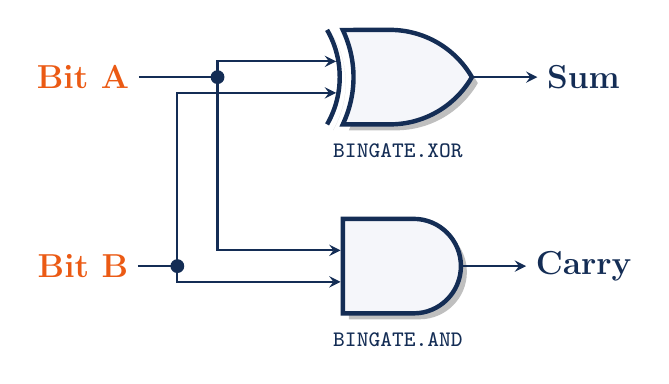
\begin{tikzpicture}[
        >=stealth,
        gate/.style={draw=DeepBlue, ultra thick, fill=LightGray, drop shadow, minimum width=1.5cm, minimum height=1.2cm},
        xor gate/.style={gate, xor gate US},
        and gate/.style={gate, and gate US},
        input/.style={font=\large\bfseries, text=AccentOrange},
        output/.style={font=\large\bfseries, text=DeepBlue}
    ]

    % Wejścia
    \node[input] (A) at (0, 1.2) {Bit A};
    \node[input] (B) at (0, -1.2) {Bit B};

    % Klasyczne bramki
    \node[xor gate] (xor) at (4, 1.2) {};
    \node[and gate] (and) at (4, -1.2) {};

    % Etykiety bramek dla OpenFHE
    \node[below=0.1cm of xor, font=\footnotesize, text=DeepBlue] {\texttt{BINGATE.XOR}};
    \node[below=0.1cm of and, font=\footnotesize, text=DeepBlue] {\texttt{BINGATE.AND}};

    % Wyjścia
    \node[output, right=0.8cm of xor] (sum) {Sum};
    \node[output, right=0.8cm of and] (carry) {Carry};

    % Wykreślanie połączeń elektronicznych - Sygnał A
    \draw[thick, DeepBlue] (A.east) -- ++(1,0) coordinate (dotA);
    \draw[->, thick, DeepBlue] (dotA) |- (xor.input 1);
    \draw[->, thick, DeepBlue] (dotA) |- (and.input 1);
    \fill[DeepBlue] (dotA) circle (2.5pt);

    % Wykreślanie połączeń elektronicznych - Sygnał B
    \draw[thick, DeepBlue] (B.east) -- ++(0.5,0) coordinate (dotB);
    \draw[->, thick, DeepBlue] (dotB) |- (and.input 2);
    \draw[->, thick, DeepBlue] (dotB) |- (xor.input 2);
    \fill[DeepBlue] (dotB) circle (2.5pt);

    % Linie wyjściowe
    \draw[->, thick, DeepBlue] (xor.output) -- (sum.west);
    \draw[->, thick, DeepBlue] (and.output) -- (carry.west);

    \end{tikzpicture}
    }
    \end{center}
\end{column}

% Prawa kolumna: Instrukcja zadania
\begin{column}{0.52\textwidth}
    \begin{block}{\faKeyboard \ Task: Encrypted Half-Adder}
        \small % Zmniejszenie czcionki tylko wewnątrz bloku
        Write a Python script using \texttt{openfhe-python} to implement the Half-Adder circuit on encrypted data!
        \vspace{0.1cm}
        \begin{itemize}
            \setlength{\itemsep}{0.05cm} % Ściśnięcie punktów w pionie
            \item[\textbf{1.}] \textbf{Setup:} Create \texttt{BinFHEContext} and generate secret \& bootstrapping keys.
            \item[\textbf{2.}] \textbf{Loop:} Iterate 4 inputs: \texttt{(0,0)} to \texttt{(1,1)}.
            \item[\textbf{3.}] \textbf{Encrypt} the inputs A and B.
            \item[\textbf{4.}] \textbf{Evaluate} homomorphically:
            \begin{itemize}
                \setlength{\itemsep}{0cm}
                \item \texttt{Sum} = \texttt{EvalBinGate(BINGATE.XOR,...)}
                \item \texttt{Carry} = \texttt{EvalBinGate(BINGATE.AND,...)}
            \end{itemize}
            \item[\textbf{5.}] \textbf{Decrypt} the outputs and print results.
        \end{itemize}
    \end{block}
\end{column}

\end{columns}
\end{frame}


% ==========================================
\begin{frame}{Time for Practice: The "Mystery Circuit"}
\begin{columns}[T]

% Lewa kolumna: Schemat
\begin{column}{0.5\textwidth}
    \vspace{0.1cm}
    \textbf{\Large What does this circuit do?} \\
    \vspace{0.3cm}
    \begin{center}
    \resizebox{0.95\textwidth}{!}{
    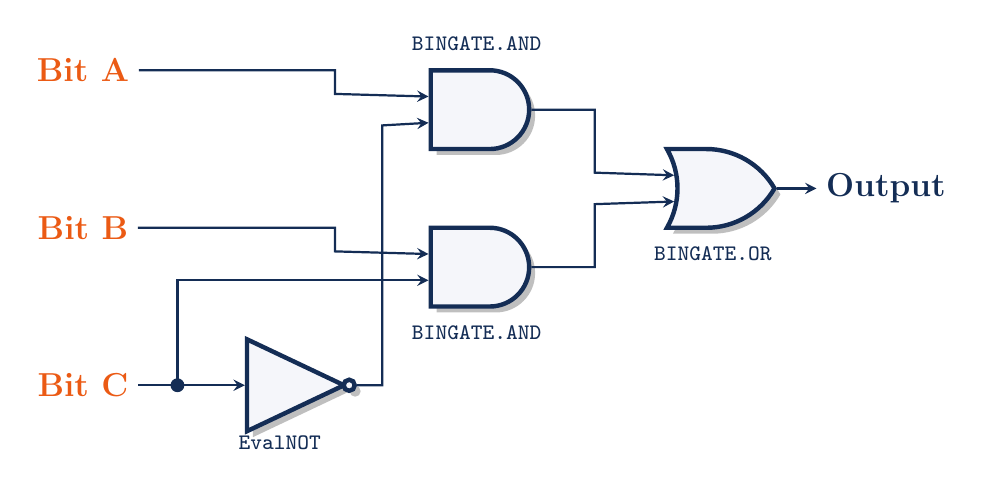
\begin{tikzpicture}[
        >=stealth,
        gate/.style={draw=DeepBlue, ultra thick, fill=LightGray, drop shadow, minimum width=1.2cm, minimum height=1cm},
        and gate/.style={gate, and gate US},
        or gate/.style={gate, or gate US},
        not gate/.style={gate, not gate US, minimum width=0.8cm},
        input/.style={font=\large\bfseries, text=AccentOrange},
        output/.style={font=\large\bfseries, text=DeepBlue}
    ]

    % Wejścia
    \node[input] (A) at (0, 2) {Bit A};
    \node[input] (B) at (0, 0) {Bit B};
    \node[input] (C) at (0, -2) {Bit C};

    % Bramki (NOT obniżone do poziomu Y=-2)
    \node[not gate] (not) at (2.5, -2) {};
    \node[and gate] (and1) at (5, 1.5) {};
    \node[and gate] (and2) at (5, -0.5) {};
    \node[or gate] (or) at (8, 0.5) {};

    % Etykiety bramek (Pomoc dla studentów)
    \node[below=0.1cm of not, font=\footnotesize, text=DeepBlue] {\texttt{EvalNOT}};
    \node[above=0.1cm of and1, font=\footnotesize, text=DeepBlue] {\texttt{BINGATE.AND}};
    \node[below=0.1cm of and2, font=\footnotesize, text=DeepBlue] {\texttt{BINGATE.AND}};
    \node[below=0.1cm of or, font=\footnotesize, text=DeepBlue] {\texttt{BINGATE.OR}};

    % --- PRECYZYJNE, BEZKOLIZYJNE LINIE ---
    
    % Sygnał A -> AND1
    \draw[->, thick, DeepBlue] (A.east) -- (3.2, 2) -- (3.2, 1.7) -- (and1.input 1);

    % Sygnał B -> AND2
    \draw[->, thick, DeepBlue] (B.east) -- (3.2, 0) -- (3.2, -0.3) -- (and2.input 1);

    % Sygnał C -> NOT oraz AND2 (omijanie od góry)
    \draw[thick, DeepBlue] (C.east) -- (1.2, -2) coordinate (dotC);
    \fill[DeepBlue] (dotC) circle (2.5pt); % Główny węzeł C
    
    % Ścieżka w górę do AND2 (|- oznacza idź pionowo, potem poziomo do celu)
    \draw[->, thick, DeepBlue] (dotC) |- (and2.input 2);
    % Ścieżka pozioma bezpośrednio do NOT
    \draw[->, thick, DeepBlue] (dotC) -- (not.input);

    % Wyjście z NOT -> AND1 (pionowy pionierski przewód na X=3.8)
    \draw[->, thick, DeepBlue] (not.output) -- (3.8, -2) -- (3.8, 1.3) -- (and1.input 2);

    % Wyjścia z AND -> OR
    \draw[->, thick, DeepBlue] (and1.output) -- (6.5, 1.5) -- (6.5, 0.7) -- (or.input 1);
    \draw[->, thick, DeepBlue] (and2.output) -- (6.5, -0.5) -- (6.5, 0.3) -- (or.input 2);

    % Wyjście końcowe
    \node[output, right=0.5cm of or] (out) {Output};
    \draw[->, thick, DeepBlue] (or.output) -- (out.west);

    \end{tikzpicture}
    }
    \end{center}
\end{column}

% Prawa kolumna: Instrukcja zadania
\begin{column}{0.48\textwidth}
    \begin{block}{\faUserSecret \ Task 2: Reverse Engineering}
        \vspace*{0.5ex}
        \footnotesize
        Implement the circuit using OpenFHE! Loop all \textbf{8 input combinations} (from \texttt{000} to \texttt{111}).
        \begin{itemize}
            \setlength{\itemsep}{0pt}
            \item Encrypt inputs A, B, and C.
            \item Evaluate the 4 gates step-by-step.
            \item Decrypt and print the final output.
        \end{itemize}
    \end{block}
    
    \begin{exampleblock}{\faQuestionCircle \ Questions to Answer}
        \vspace*{0.5ex}
        \footnotesize
        Analyze the truth table in your console:
        \begin{itemize}
            \setlength{\itemsep}{0.1cm}
            \item[\textbf{1.}] What role does \textbf{Bit C} play?
            \item[\textbf{2.}] What fundamental programming construct does this circuit replace in FHE?
        \end{itemize}
    \end{exampleblock}
\end{column}

\end{columns}
\end{frame}


\begin{frame}[fragile]{Solution: The FHE "IF-ELSE" Statement}
\begin{columns}[T]

% Lewa kolumna: Analiza tabeli prawdy
\begin{column}{0.45\textwidth}
    \begin{block}{\faTable \ Truth Table Analysis}
        \vspace*{0.5ex}
        \footnotesize
        \centering
        \renewcommand{\arraystretch}{0.9} % Ściśnięcie tabeli w pionie
        \begin{tabular}{ccc|c}
            \textbf{C (Control)} & \textbf{Bit A} & \textbf{Bit B} & \textbf{Output} \\
            \hline
            \textcolor{red}{\textbf{0}} & 0 & 0 & \textbf{0} \\
            \textcolor{red}{\textbf{0}} & 0 & 1 & \textbf{0} \\
            \textcolor{red}{\textbf{0}} & 1 & 0 & \textbf{1} \\
            \textcolor{red}{\textbf{0}} & 1 & 1 & \textbf{1} \\
            \hline
            \textcolor{green!60!black}{\textbf{1}} & 0 & 0 & \textbf{0} \\
            \textcolor{green!60!black}{\textbf{1}} & 0 & 1 & \textbf{1} \\
            \textcolor{green!60!black}{\textbf{1}} & 1 & 0 & \textbf{0} \\
            \textcolor{green!60!black}{\textbf{1}} & 1 & 1 & \textbf{1} \\
        \end{tabular}
        \vspace{0.15cm}
        \begin{itemize}
            \setlength{\itemsep}{0pt}
            \item When \textbf{C = 0}, Output = \textbf{Bit A}
            \item When \textbf{C = 1}, Output = \textbf{Bit B}
        \end{itemize}
    \end{block}
\end{column}

% Prawa kolumna: Wyjaśnienie MUX
\begin{column}{0.52\textwidth}
    \begin{exampleblock}{\faLightbulb \ The Multiplexer (MUX)}
        \vspace*{0.5ex}
        \footnotesize
        You built a \textbf{MUX}, the FHE equivalent of conditional logic: \\
        \vspace{0.1cm}
        \texttt{\textcolor{DeepBlue}{if} (C == 1) \textcolor{DeepBlue}{return} B; \textcolor{DeepBlue}{else return} A;}
        \vspace{0.2cm}
        
        \textbf{Why is this crucial?} \\
        The cloud cannot read encrypted \texttt{C}, making standard \texttt{if-else} branching impossible! 
        \vspace{0.1cm}
        
        Instead, it computes \textbf{both} branches and mathematically filters the result.
    \end{exampleblock}
    
    \begin{alertblock}{\faMicrochip \ Native CMUX Gate}
        \vspace*{0.5ex}
        \footnotesize
        OpenFHE provides a native, optimized gate for this: \\
        \texttt{EvalBinGate(BINGATE.CMUX, [C, B, A])}
    \end{alertblock}
\end{column}

\end{columns}
\end{frame}

\section{BFV Scheme}
\begin{frame}{2. BFV Scheme}
\begin{columns}[T]
\begin{column}{0.25\textwidth}
    \vspace{0.5cm}
    \centering
    \textcolor{DeepBlue}{\Huge \faCalculator} \\ \vspace{0.3cm}
    \textcolor{AccentOrange}{\Large \faListOl}
\end{column}
\begin{column}{0.7\textwidth}
    \Large \textbf{Exact Integer Arithmetic} \\
    \normalsize \vspace{0.3cm}
    \begin{itemize}
        \item Optimized for exact operations on \textbf{integers}.
        \item Supports \textbf{SIMD Batching}: efficiently packing arrays of numbers into a single ciphertext for parallel computation.
        \item \textbf{Best for:} Financial computing, exact statistics, database queries.
    \end{itemize}
\end{column}
\end{columns}
\end{frame}

% --- SLAJD 1: BFV Setup - Parameters ---
\begin{frame}[fragile]{BFV Setup (1/3): Parameters \& Context}
\vspace{0.1cm}
\begin{lstlisting}[firstnumber=1]
from openfhe import *

# 1. Setup CryptoContext for BFV
# Container for BFV parameters (operates on integer vectors).
parameters = CCParamsBFVRNS()

# Plaintext modulus (t). Defines the max range of numbers 
# we can pack into the vector before encryption.
parameters.SetPlaintextModulus(65537)

# Allocates "noise budget". A depth of 2 allows the cloud to 
# perform 2 sequential vector multiplications safely.
parameters.SetMultiplicativeDepth(2)

# Creates the main environment manager for all FHE operations.
crypto_context = GenCryptoContext(parameters)
\end{lstlisting}
\end{frame}

% --- SLAJD 2: BFV Setup - Enabling Features ---
\begin{frame}[fragile]{BFV Setup (2/3): Enabling Features}
\vspace{0.1cm}
\begin{lstlisting}[firstnumber=8]
# By default, OpenFHE disables all features to save memory. 
# We must explicitly enable the cryptographic capabilities we need.

# Unlocks basic cryptographic operations: key generation, 
# encryption (Encrypt), and decryption (Decrypt).
crypto_context.Enable(PKESchemeFeature.PKE)

# Enables Key Switching. This is a core mechanism absolutely 
# necessary for vector multiplication and rotation in the cloud.
crypto_context.Enable(PKESchemeFeature.KEYSWITCH)

# Unlocks homomorphic mathematical operations on the server, 
# giving us access to methods like EvalAdd and EvalMult.
crypto_context.Enable(PKESchemeFeature.LEVELEDSHE)
\end{lstlisting}
\end{frame}

% --- SLAJD 3: BFV Setup - Key Generation ---
\begin{frame}[fragile]{BFV Setup (3/3): Key Generation}
\vspace{0.1cm}
\begin{lstlisting}[firstnumber=13]
# ==========================================
# Key Generation
# ==========================================

# KeyGen() returns a KeyPair object containing the standard 
# private key (for decryption) and public key (for encryption).
key_pair = crypto_context.KeyGen()

# Multiplying ciphertexts makes them grow too large to handle. 
# EvalMultKeyGen() creates a special "Multiplication Key".
# It allows the cloud server to mathematically "compress" the 
# result back to its normal size after each multiplication.
# This keeps computations fast, without exposing your secret key!
crypto_context.EvalMultKeyGen(key_pair.secretKey) 
\end{lstlisting}
\end{frame}

% --- SLAJD 2: BFV Encoding & Encryption ---
\begin{frame}[fragile]{BFV: SIMD Encoding \& Encrypt (Client)}
\vspace{0.1cm}
\begin{lstlisting}[firstnumber=18]
# ==========================================
# SIMD Encoding & Encryption
# ==========================================
vec_a = [ 2, 4, 6, 8 ]
vec_b = [ 3, 2, 1, 5 ]

# Packs the integer arrays into single Plaintext objects.
# This enables SIMD Batching: packing multiple numbers into one
# structure to perform parallel FHE operations on all of them.
ptxt_a = crypto_context.MakePackedPlaintext(vec_a)
ptxt_b = crypto_context.MakePackedPlaintext(vec_b)

# Encrypts the packed plaintexts using the Public Key.
# The resulting ciphertexts can now be safely sent to the cloud.
ctxt_a = crypto_context.Encrypt(key_pair.publicKey, ptxt_a)
ctxt_b = crypto_context.Encrypt(key_pair.publicKey, ptxt_b)
\end{lstlisting}
\end{frame}


% --- SLAJD 3: BFV Evaluation (Cloud) ---
\begin{frame}[fragile]{BFV: Evaluation (Cloud)}
\vspace{0.1cm}
\begin{lstlisting}[firstnumber=29]
# ==========================================
# Homomorphic Evaluation (Cloud)
# ==========================================
# The ciphertexts are sent to the untrusted cloud. 
# The server computes on them without ever knowing the 
# underlying plaintext data or the secret key.

print("Evaluating EvalMult on encrypted vectors...")

# EvalMult multiplies ALL corresponding elements in the 
# packed arrays simultaneously (SIMD Batching). 
# It automatically uses the Multiplication Key stored in 
# the CryptoContext to mathematically "compress" (relinearize) 
# the resulting ciphertext back to its normal size.
ctxt_result = crypto_context.EvalMult(ctxt_a, ctxt_b)
\end{lstlisting}
\end{frame}

% --- SLAJD 4: BFV Decryption ---
\begin{frame}[fragile]{BFV: Decrypt \& Extract (Client)}
\vspace{0.1cm}
\begin{lstlisting}[firstnumber=38]
# ==========================================
# Decrypt & Extract (Client)
# ==========================================
# The cloud returns the evaluated ciphertext. The client 
# decrypts it using their secret key to recover the Plaintext.

result_ptxt = crypto_context.Decrypt(key_pair.secretKey, ctxt_result)

# GetPackedValue() extracts the underlying vector from the 
# Plaintext object. We slice [:4] to see only our actual 
# data, ignoring the padding zeros added by the ring dimension.

print(f"Decrypted Result: {result_ptxt.GetPackedValue()[:4]}")

# Expected Console Output:
# Decrypted Result: [ 6,  8,  6,  40 ]
\end{lstlisting}
\end{frame}


% --- SLAJD 1: BGV & Bootstrapping (Problem) ---
\begin{frame}{BGV: The Missing Bootstrapping (1/2)}
\Large \textbf{Why doesn't BGV have an EvalBootstrap() method?} \\
\vspace{0.4cm}
\normalsize
BGV is an exact integer scheme. While a bootstrapping algorithm theoretically exists for it (based on \textit{digit extraction}), it has a \textbf{terrifying computational complexity}. Because of this extreme overhead, OpenFHE does NOT expose it in its standard API.

\vspace{0.5cm}
\begin{alertblock}{\faExclamationTriangle \ The Danger of Deep Circuits}
    Without bootstrapping, we cannot "refresh" the noise on the fly mid-computation. If we multiply ciphertexts too many times, the noise explosion will irreversibly destroy the data!
\end{alertblock}
\end{frame}

% --- SLAJD 2: BGV & Bootstrapping (Rozwiązanie) ---
\begin{frame}{BGV: The Missing Bootstrapping (2/2)}
\Large \textbf{How do we compute without Bootstrapping?} \\
\vspace{0.4cm}
\normalsize
Since we cannot reset the cryptographic noise in the cloud, we must plan our entire circuit's depth before the encryption even begins.

\vspace{0.5cm}
\begin{exampleblock}{\faCheckCircle \ The OpenFHE Solution: Pre-allocation}
    Instead of relying on bootstrapping, developers must define a strict noise budget upfront using the \textbf{\texttt{MultiplicativeDepth}} parameter. This dictates exactly how many sequential multiplications the cloud can safely perform before the data is lost.
\end{exampleblock}
\end{frame}

% --- SLAJD 1: BGV Multiplicative Depth (Kod 1/2) ---
\begin{frame}[fragile]{BGV in Practice: Multiplicative Depth (1/2)}
\vspace{0.1cm}
\begin{lstlisting}[firstnumber=1]
def run_bgv_scenario(depth: int, num_multiplications: int):
    # 1. Setup: Define the maximum sequential multiplications
    parameters = CCParamsBGVRNS()
    parameters.SetMultiplicativeDepth(depth)
    
    # ... (GenCryptoContext, KeyGen, Encrypt vector) ...
    
    current_ctxt = ctxt # <-- it's an encrypted vector [1,2,3,4]
    
    # 2. Evaluation: Each EvalMult consumes the depth budget!
    for i in range(num_multiplications):
        current_ctxt = crypto_context.EvalMult(current_ctxt, ctxt)

    # 3. Decryption
    result = crypto_context.Decrypt(key_pair.secretKey, current_ctxt)
    print(f"Decrypted: {result.GetPackedValue()[:4]}\n")
\end{lstlisting}
\end{frame}

% --- SLAJD 2: BGV Multiplicative Depth (Kod 2/2) ---
\begin{frame}[fragile]{BGV in Practice: Multiplicative Depth (2/2)}
\vspace{0.1cm}
\begin{lstlisting}[firstnumber=24]
if __name__ == "__main__":
    # -------------------------------------------------------------
    # Scenario 1: Budget exceeded
    # -------------------------------------------------------------
    # We allocate a budget for 1 multiplication, but perform 2.
    # The noise explosion will irrevocably corrupt the data (garbage)
    print("--- BGV test with MultiplicativeDepth = 1 ---")
    run_bgv_scenario(depth=1, num_multiplications=2)
    
    # -------------------------------------------------------------
    # Scenario 2: Budget adjusted (The OpenFHE Solution for BGV)
    # -------------------------------------------------------------
    # Since OpenFHE does not support EvalBootstrap() for BGV, 
    # we must correctly allocate the noise budget in advance.
    print("--- BGV test with MultiplicativeDepth = 2 ---")
    run_bgv_scenario(depth=2, num_multiplications=2)
\end{lstlisting}
\end{frame}

% --- SLAJD: BGV Console Output ---
\begin{frame}[fragile]{BGV in Practice: Console Output}
\vspace{0.1cm}

\begin{alertblock}{\faExclamationTriangle \ Scenario 1: Budget Exceeded (Depth = 1)}
\begin{lstlisting}[language={}, basicstyle=\ttfamily\small\color{white}, backgroundcolor=\color{black!85}, numbers=none]
--- BGV test with MultiplicativeDepth = 1 ---
Original vector: [1, 2, 3, 4]
Performing multiplication 1...
Performing multiplication 2...
Decrypted result: [-26843, -16257, 702, 2507]
\end{lstlisting}
\end{alertblock}
\end{frame}

% --- SLAJD: BGV Console Output ---
\begin{frame}[fragile]{BGV in Practice: Console Output}
\vspace{0.1cm}

\begin{exampleblock}{\faCheckCircle \ Scenario 2: Budget Adjusted (Depth = 2)}
\begin{lstlisting}[language={}, basicstyle=\ttfamily\small\color{white}, backgroundcolor=\color{black!85}, numbers=none]
--- BGV test with MultiplicativeDepth = 2 ---
Original vector: [1, 2, 3, 4]
Performing multiplication 1...
Performing multiplication 2...
Decrypted result: [1, 8, 27, 64]
\end{lstlisting}
\end{exampleblock}

\end{frame}

% --- SLAJD: Polynomial Evaluation Example ---
\begin{frame}{Polynomial Evaluation Example}
\large \textbf{Computing $f(x) = 2x^2 + 3x + 1$ in Parallel} \\
\vspace{0.1cm}
\small
The \textbf{BGV} scheme encodes data in packed vectors. When we evaluate the polynomial homomorphically, the cloud uses \textbf{SIMD} (\textit{Single Instruction, Multiple Data}) architecture. This means the exact same mathematical operations are applied to all encrypted slots simultaneously!

\vspace{0.1cm}
\begin{center}
\resizebox{0.7\textwidth}{!}{
\begin{tikzpicture}[
    >=stealth,
    slot/.style={draw=DeepBlue, thick, fill=white, minimum width=2.0cm, minimum height=0.6cm, align=center, font=\Large\bfseries},
    outslot/.style={draw=mygreen, thick, fill=mygreen!10, minimum width=2.0cm, minimum height=0.6cm, align=center, font=\Large\bfseries},
    cloud/.style={draw=AccentOrange, thick, fill=AccentOrange!10, rounded corners=8pt, minimum width=8.6cm, minimum height=0.9cm, align=center, font=\Large\bfseries, dashed, drop shadow},
    arrow/.style={->, ultra thick, DeepBlue}
]

% Input Vector (Multiple Data)
\node[slot] (x0) at (0, 0) {$x_0$};
\node[slot] (x1) at (2.2, 0) {$x_1$};
\node[slot] (x2) at (4.4, 0) {$x_2$};
\node[slot] (x3) at (6.6, 0) {$x_3$};

\node[left=0.2cm of x0, font=\Large\bfseries, DeepBlue] {\faLock \ Enc};

% Brace for Multiple Data
\draw[thick, DeepBlue, decorate, decoration={brace, amplitude=5pt}] (-1.1, 0.4) -- (7.7, 0.4) node[midway, above=0.15cm, font=\large\bfseries] {Multiple Data};

% Cloud Operation (Single Instruction)
\node[cloud] (fhe) at (3.3, -1.3) {\faCloud \ $f(x) = 2x^2 + 3x + 1$};
\node[right=0.2cm of fhe, font=\large\bfseries, AccentOrange, align=left] {Single \\ Instruction};

% Output Vector
\node[outslot] (y0) at (0, -2.6) {$f(x_0)$};
\node[outslot] (y1) at (2.2, -2.6) {$f(x_1)$};
\node[outslot] (y2) at (4.4, -2.6) {$f(x_2)$};
\node[outslot] (y3) at (6.6, -2.6) {$f(x_3)$};

\node[left=0.2cm of y0, font=\Large\bfseries, mygreen] {\faLock \ Enc};

% Arrows down (Input to Cloud)
\draw[arrow] (x0.south) -- (x0.south |- fhe.north);
\draw[arrow] (x1.south) -- (x1.south |- fhe.north);
\draw[arrow] (x2.south) -- (x2.south |- fhe.north);
\draw[arrow] (x3.south) -- (x3.south |- fhe.north);

% Arrows down (Cloud to Output)
\draw[arrow] (x0.south |- fhe.south) -- (y0.north);
\draw[arrow] (x1.south |- fhe.south) -- (y1.north);
\draw[arrow] (x2.south |- fhe.south) -- (y2.north);
\draw[arrow] (x3.south |- fhe.south) -- (y3.north);

\end{tikzpicture}
}
\end{center}
\end{frame}

% --- SLAJD 1: Polynomial Evaluation (Configuration) ---
\begin{frame}[fragile]{Evaluating $f(x) = 2x^2 + 3x + 1$ (BGV CryptoContext Configuration)}
\vspace{0.1cm}
\begin{lstlisting}[firstnumber=1]
from openfhe import *

parameters = CCParamsBGVRNS()
parameters.SetPlaintextModulus(65537)
    
# We reserve a multiplicative depth of 2:
# - 1 level for EvalSquare (x^2)
# - 1 level for EvalMult (multiplying x^2 by the constant 2)
parameters.SetMultiplicativeDepth(2) 
crypto_context = GenCryptoContext(parameters)
\end{lstlisting}
\end{frame}

% --- SLAJD 2: Polynomial Evaluation (Enabling Features) ---
\begin{frame}[fragile]{Evaluating $f(x) = 2x^2 + 3x + 1$ (BGV CryptoContext Configuration)}
\vspace{0.1cm}
\begin{lstlisting}[firstnumber=11]
# Enable features required for our operations:
# PKE (Public Key Encryption): Enables basic cryptographic 
# functions like KeyGen(), Encrypt(), and Decrypt().
crypto_context.Enable(PKESchemeFeature.PKE)
    
# KEYSWITCH: Enables key switching. This is crucial for 
# relinearization (flattening the ciphertext back to its 
# normal size after EvalSquare or EvalMult).
crypto_context.Enable(PKESchemeFeature.KEYSWITCH)
    
# LEVELEDSHE: Enables mathematical operations on ciphertexts 
# (EvalAdd, EvalMult, EvalSquare) within the depth budget.
crypto_context.Enable(PKESchemeFeature.LEVELEDSHE)
\end{lstlisting}
\end{frame}

% --- SLAJD 3: Polynomial Evaluation (Keys & Encryption) ---
\begin{frame}[fragile]{Evaluating $f(x) = 2x^2 + 3x + 1$ (Key Generation)}
\vspace{0.1cm}
\begin{lstlisting}[firstnumber=24]
key_pair = crypto_context.KeyGen()
    
# EvalMultKeyGen generates evaluation keys (relinearization keys).
# This is absolutely required before calling EvalSquare() or EvalMult(), 
# allowing the cloud to compute products securely.
crypto_context.EvalMultKeyGen(key_pair.secretKey)
key_pair = crypto_context.KeyGen()
\end{lstlisting}
\end{frame}

% --- SLAJD 3: Polynomial Evaluation (Keys & Encryption) ---
\begin{frame}[fragile]{Evaluating $f(x) = 2x^2 + 3x + 1$ (Data Encryption)}
\vspace{0.1cm}
\begin{lstlisting}[firstnumber=31]
vec = [1, 2, 3, 4]
    
# Pack the vector into a Plaintext object to compute in SIMD mode
ptxt = crypto_context.MakePackedPlaintext(vec)
ctxt = crypto_context.Encrypt(key_pair.publicKey, ptxt)
\end{lstlisting}
\end{frame}

% --- SLAJD 4: Polynomial Evaluation (SIMD Encoding) ---
\begin{frame}[fragile]{Evaluating $f(x) = 2x^2 + 3x + 1$ (Encoding Constants as Plaintexts)}
\vspace{0.1cm}
\begin{lstlisting}[firstnumber=36]
# In BGV (SIMD mode), we cannot multiply a ciphertext directly 
# by a raw integer scalar. We must duplicate each constant across 
# the entire length of the input vector and encode them as 
# Plaintext objects so SIMD operations work on every slot.
    
vec_len = len(vec)
    
ptxt_2 = crypto_context.MakePackedPlaintext([2] * vec_len) # Creates [2, 2, 2, 2]
ptxt_3 = crypto_context.MakePackedPlaintext([3] * vec_len) # Creates [3, 3, 3, 3]
ptxt_1 = crypto_context.MakePackedPlaintext([1] * vec_len) # Creates [1, 1, 1, 1]
\end{lstlisting}
\end{frame}

% --- SLAJD 5: Polynomial Evaluation (Circuit Evaluation) ---
\begin{frame}[fragile]{Evaluating $f(x) = 2x^2 + 3x + 1$ (Manual Polynomial Evaluation in BGV)}
\vspace{0.1cm}
\begin{lstlisting}[firstnumber=46]
# STEP A: x^2 (Consumes 1 level of multiplicative depth)
ctxt_x2 = crypto_context.EvalSquare(ctxt)
    
# STEP B: 2 * x^2 (Consumes 1 level of multiplicative depth)
ctxt_2x2 = crypto_context.EvalMult(ctxt_x2, ptxt_2)
    
# STEP C: 3 * x
ctxt_3x = crypto_context.EvalMult(ctxt, ptxt_3)
    
# STEP D: (2x^2) + (3x) (EvalAdd adds very little noise)
ctxt_res = crypto_context.EvalAdd(ctxt_2x2, ctxt_3x)
    
# STEP E: Adding the constant 1 at the end: + 1
ctxt_res = crypto_context.EvalAdd(ctxt_res, ptxt_1)
\end{lstlisting}
\end{frame}

% --- SLAJD 6: Polynomial Evaluation (Decryption & Output) ---
\begin{frame}[fragile]{Evaluating $f(x) = 2x^2 + 3x + 1$ (Decryption of the Results)}
\vspace{0.3cm}
\begin{lstlisting}[firstnumber=60]
result_ptxt = crypto_context.Decrypt(key_pair.secretKey, ctxt_res)
    
# Extract only the valid elements (ignoring trailing zeros)
result_vec = result_ptxt.GetPackedValue()[:vec_len]
    
print(f"Decrypted result: {result_vec}\n")
\end{lstlisting}
\end{frame}

% --- SLAJD 7: Polynomial Evaluation (Results) ---
\begin{frame}[fragile]{Evaluating $f(x) = 2x^2 + 3x + 1$ (Results)}
\vspace{0.1cm}

\begin{exampleblock}{\faTerminal \ Console Output}
\begin{lstlisting}[language={}, basicstyle=\ttfamily\scriptsize\color{white}, backgroundcolor=\color{black!85}, numbers=none]
Original vector: [0, 1, 2, 3]
Computing polynomial manually: f(x) = 2x^2 + 3x + 1
Decrypted result: [1, 6, 15, 28]
\end{lstlisting}
\end{exampleblock}

\vspace{0.2cm}
\large \textbf{\textcolor{mygreen}{\faCheckCircle} \ Math Verification (SIMD in action):} \\
\small
\vspace{0.1cm}
Notice how the cloud correctly evaluated the polynomial for all slots simultaneously:

\vspace{0.1cm}
\begin{columns}
    \begin{column}{0.48\textwidth}
        \begin{itemize}
            \item \textcolor{DeepBlue}{$f(0)$} $= 2(0)^2 + 3(0) + 1 =$ \textbf{1}
            \item \textcolor{DeepBlue}{$f(1)$} $= 2(1)^2 + 3(1) + 1 =$ \textbf{6}
        \end{itemize}
    \end{column}
    \begin{column}{0.48\textwidth}
        \begin{itemize}
            \item \textcolor{DeepBlue}{$f(2)$} $= 2(2)^2 + 3(2) + 1 =$ \textbf{15}
            \item \textcolor{DeepBlue}{$f(3)$} $= 2(3)^2 + 3(3) + 1 =$ \textbf{28}
        \end{itemize}
    \end{column}
\end{columns}

\end{frame}

\begin{frame}{Time for Practice: Secure Polynomial Evaluation (BGV)}
\begin{block}{\faKeyboard \ Task: Cloud Risk Assessment using SIMD}
\small
Write a Python script using \texttt{openfhe-python} to evaluate the risk function $f(x) = x^4 + 2x^3 + 3x^2 + 4$ on a batch of patients $x = [0, 7, 12, 2]$ using the BGV scheme.
\vspace{0.1cm}
\begin{itemize}
\setlength{\itemsep}{0.05cm}
\item[\textbf{1.}] \textbf{Calculate Depth:} Manually determine the exact \texttt{MultiplicativeDepth} required to evaluate the polynomial.
\item[\textbf{2.}] \textbf{Setup:} Configure \texttt{CCParamsBGVRNS} with \texttt{PlaintextModulus=65537}. Enable necessary features (PKE, KEYSWITCH, LEVELEDSHE) and generate the \texttt{EvalMultKey}.
\item[\textbf{3.}] \textbf{SIMD Packing:} Encode the input vector and the constants (2, 3, and 4) as packed vectors across all slots using \texttt{MakePackedPlaintext}.
\item[\textbf{4.}] \textbf{Evaluate \& Verify:} Compute $f(x)$ homomorphically using \texttt{EvalSquare}, \texttt{EvalMult}, and \texttt{EvalAdd}. Decrypt and extract the result.
\end{itemize}
\end{block}
\end{frame}

% --- SLAJD: E-Voting System Task ---
\begin{frame}{Time for Practice: Secure E-Voting System}
\begin{columns}[T]

% Lewa kolumna: Koncepcja i wizualizacja
\begin{column}{0.43\textwidth}
\vspace{0.1cm}
\textbf{\large The Voting Scenario} \\
\vspace{0.3cm}
\small
\begin{itemize}
    \item \textbf{Voters:} Each voter casts a vote as a vector. They encrypt it using the \textbf{Public Key} (\texttt{PKE}).
    \item \textbf{Cloud Server:} Receives encrypted votes and homomorphically sums them without decrypting or knowing the private key.
    \item \textbf{Election Committee:} Uses the \textbf{Secret Key} to decrypt the final sum.
\end{itemize}
\vspace{0.4cm}
\begin{center}
% Wizualizacja przepływu używająca ikon fontawesome5
\textcolor{DeepBlue}{\LARGE \faUsers} \quad \textcolor{AccentOrange}{\LARGE \faArrowRight} \quad \textcolor{DeepBlue}{\LARGE \faCloud} \quad \textcolor{AccentOrange}{\LARGE \faArrowRight} \quad \textcolor{mygreen}{\LARGE \faUnlock}
\end{center}
\end{column}

% Prawa kolumna: Instrukcja zadania
\begin{column}{0.54\textwidth}
\begin{block}{\faKeyboard \ Task: Encrypted Summing in BGV}
\footnotesize
Write a Python script using \texttt{openfhe-python} to implement the E-Voting system!
\vspace{0.1cm}
\begin{itemize}
    \setlength{\itemsep}{0pt}
    \item \textbf{Setup:} Create \texttt{CCParamsBGVRNS}, set depth to 2, and enable \texttt{PKE} and \texttt{LEVELEDSHE}.
    \item \textbf{KeyGen:} Generate a \texttt{KeyPair} for the election.
    \item \textbf{Encrypt:} Loop through 5 simulated vote vectors. Encode them using \texttt{MakePackedPlaintext} and encrypt using the \textbf{Public Key}.
    \item \textbf{Evaluate:} Sum the votes sequentially using \texttt{EvalAdd}.
    \item \textbf{Decrypt:} Decrypt the sum with the \textbf{Private Key}, restrict the length to 5 using \texttt{SetLength(5)}, and print the final sum.
\end{itemize}
\end{block}
\end{column}

\end{columns}
\end{frame}

% --- SLAJD: Praktyczne ćwiczenie z BFV i EvalInnerProduct ---
\begin{frame}{Time for Practice: Secure Portfolio Valuation (BFV)}
\begin{columns}[T]
% Lewa kolumna: Scenariusz
\begin{column}{0.46\textwidth}
\vspace{0.1cm}
\textbf{\large The Scenario} \\
\vspace{0.2cm}
\small
A client holds a portfolio of exactly 4 assets and wants the cloud server to compute its total value based on current market prices.
\vspace{0.2cm}
\begin{itemize}
\setlength{\itemsep}{0.1cm}
\item \textbf{Client:} Encrypts the quantities of the assets (e.g., \texttt{[1, 2, 0, 11]}).
\item \textbf{Server:} Holds the current market prices in plaintext (e.g., \texttt{[10, 3, 4, 2]}).
\item \textbf{Goal:} Use SIMD batching and the homomorphic Dot Product operation to compute the final value securely.
\end{itemize}
\end{column}

% Prawa kolumna: Instrukcja zadania
\begin{column}{0.53\textwidth}
\begin{block}{\faKeyboard \ Task: BFV Inner Product}
\footnotesize
Write a Python script using \texttt{openfhe-python} to implement this computation!
\begin{itemize}
\setlength{\itemsep}{0.05cm}
\item[\textbf{1.}] \textbf{Setup:} Configure \texttt{CCParamsBFVRNS}. Set \texttt{PlaintextModulus} to 65537, \texttt{MultiplicativeDepth} to 2, and crucially, \texttt{BatchSize} to 4.
\item[\textbf{2.}] \textbf{Enable Features:} Enable \texttt{PKE}, \texttt{KEYSWITCH}, \texttt{LEVELEDSHE}, and \texttt{ADVANCEDSHE} (required for aggregation).
\item[\textbf{3.}] \textbf{Keys:} Generate the secret/public keys, \texttt{EvalMultKey}, and \texttt{EvalSumKey}.
\item[\textbf{4.}] \textbf{Encode \& Encrypt:} Pack both vectors using \texttt{MakePackedPlaintext}. Encrypt the quantities, keep prices as Plaintext.
\item[\textbf{5.}] \textbf{Evaluate \& Decrypt:} Compute the portfolio value using \texttt{EvalInnerProduct}. Decrypt and extract the scalar result!
\end{itemize}
\end{block}
\end{column}
\end{columns}
\end{frame}

% --- SLAJD 4: Schemat CKKS ---
\section{CKKS Scheme}
\begin{frame}{3. CKKS Scheme}
\begin{columns}[T]
\begin{column}{0.25\textwidth}
    \vspace{0.5cm}
    \centering
    \textcolor{DeepBlue}{\Huge \faBrain} \\ \vspace{0.3cm}
    \textcolor{AccentOrange}{\Large \faChartLine}
\end{column}
\begin{column}{0.7\textwidth}
    \Large \textbf{Approximate Real-Number Arithmetic} \\
    \normalsize \vspace{0.3cm}
    \begin{itemize}
        \item The only scheme that natively handles \textbf{floating-point / real numbers}.
        \item It is an \textit{approximate} scheme (like floating-point math in regular CPUs, it introduces tiny rounding errors).
        \item \textbf{Best for:} Machine Learning (AI inferences), polynomial approximations, statistical modeling.
    \end{itemize}
\end{column}
\end{columns}
\end{frame}

% --- SLIDE 5: Student Task ---
\begin{frame}{CKSS Example: Secure Cloud Risk Assessment}
\begin{block}{\faKeyboard \ Encrypted AI Inference}
\small
\vspace{0.1cm}
\begin{itemize}
\setlength{\itemsep}{0.05cm}
\item[\textbf{1.}] \textbf{Scenario:} A cloud server evaluates a single artificial neuron equation: $y = \sum_{i=1}^{n} (x_i \cdot w_i) + b$.
\item[\textbf{2.}] \textbf{Encryption:} The client encrypts medical results $x_i$ as a packed floating-point vector using \texttt{MakeCKKSPackedPlaintext}.
\item[\textbf{3.}] \textbf{Evaluation:} The cloud homomorphically multiplies the encrypted features by the plaintext weights $w_i$, sums the resulting vector using \texttt{EvalSum} (remember to generate the sum key!), and adds the scalar bias $b$.
\item[\textbf{4.}] \textbf{Decryption:} The client decrypts the vector using \texttt{GetRealPackedValue} and extracts its first position to get the final risk score.
\end{itemize}
\end{block}
\end{frame}

% --- SLIDE 2a: Setup ---
\begin{frame}[fragile]{CKKS in Practice: Setup}
\vspace{0.1cm}
\begin{lstlisting}[firstnumber=1]
from openfhe import *

# 1. Setup CryptoContext for CKKS scheme
parameters = CCParamsCKKSRNS()
parameters.SetMultiplicativeDepth(1)
parameters.SetScalingModSize(50)
parameters.SetBatchSize(4)

crypto_context = GenCryptoContext(parameters)
\end{lstlisting}
\end{frame}

% --- SLIDE 2b: Features & Keys ---
\begin{frame}[fragile]{CKKS in Practice: Features \& Keys}
\vspace{0.1cm}
\begin{lstlisting}[firstnumber=11]
# Enable required features (ADVANCEDSHE is needed for EvalSum)
crypto_context.Enable(PKESchemeFeature.PKE)
crypto_context.Enable(PKESchemeFeature.KEYSWITCH)
crypto_context.Enable(PKESchemeFeature.LEVELEDSHE)
crypto_context.Enable(PKESchemeFeature.ADVANCEDSHE)

# 2. Key Generation
key_pair = crypto_context.KeyGen()
crypto_context.EvalMultKeyGen(key_pair.secretKey)
crypto_context.EvalSumKeyGen(key_pair.secretKey)
\end{lstlisting}
\end{frame}
% --- SLIDE 3a: Encoding & Encryption ---
\begin{frame}[fragile]{CKKS in Practice: Encrypt Data}
\vspace{0.1cm}
\begin{lstlisting}[firstnumber=21]
# 3. Client Side: Encrypt patient medical data
patient_features = [1.2, 3.5, 0.8, 2.1]
ptxt_features = crypto_context.MakeCKKSPackedPlaintext(patient_features)
ctxt_features = crypto_context.Encrypt(key_pair.publicKey, ptxt_features)

# 4. Cloud Side: Cloud AI Model parameters
model_weights = [0.5, -1.2, 2.0, 0.9]
bias = 0.75
ptxt_weights = crypto_context.MakeCKKSPackedPlaintext(model_weights)
\end{lstlisting}
\end{frame}

% --- SLIDE 3b: Homomorphic Evaluation ---
\begin{frame}[fragile]{CKKS in Practice: Evaluate Neural Network}
\vspace{0.1cm}
\begin{lstlisting}[firstnumber=30]
# Evaluate the neuron: y = sum(x_i * w_i) + b
# Step A: Element-wise multiplication of features and weights
ctxt_mult = crypto_context.EvalMult(ctxt_features, ptxt_weights)

# Step B: Sum all components in the packed ciphertext vector
ctxt_sum = crypto_context.EvalSum(ctxt_mult, 4)

# Step C: Add the bias (scalar addition natively supported in CKKS)
ctxt_result = crypto_context.EvalAdd(ctxt_sum, bias)
\end{lstlisting}
\end{frame}

% --- SLIDE 4: Decryption & Output Extraction ---
\begin{frame}[fragile]{CKKS in Practice: Decryption}
\vspace{0.1cm}
\begin{lstlisting}[firstnumber=40]
# 5. Client Side: Decryption
result_ptxt = crypto_context.Decrypt(key_pair.secretKey, ctxt_result)

# Extract the vector of real numbers from the plaintext
result_vec = result_ptxt.GetRealPackedValue()

# Extract only the first element as the final scalar prediction score
final_score = result_vec[0]

print(f"Encrypted Network Prediction Score: {final_score}")
\end{lstlisting}
\vspace{0.2cm}
\begin{block}{\faLightbulb \ The SIMD Effect in \texttt{EvalSum}}
\small Because \texttt{EvalSum} sums all slots and duplicates the result across the entire vector, we simply extract the very first element to retrieve the final scalar prediction.
\end{block}
\end{frame}



\begin{frame}{Work in Progress: Upcoming Materials}
\begin{columns}[T]
\begin{column}{0.95\textwidth}
    \Large \textbf{\textcolor{DeepBlue}{\faTools \ Coming Soon...}} \\
    \normalsize \vspace{0.3cm}
    The following sections are currently under development and will be added to the training materials shortly:
    \vspace{0.4cm}

    \begin{block}{\faKeyboard \ Advanced BGV Challenge}
    \small
    A more complex and engaging programming task utilizing \textbf{homomorphic vector rotations} (\texttt{EvalRotate}) and SIMD packing to compute dot products and advanced metrics under the BGV scheme.
    \end{block}

    \vspace{0.2cm}
    \begin{exampleblock}{\faBrain \ Introduction to the CKKS Scheme}
    \small
    A comprehensive section on \textbf{Approximate Real-Number Arithmetic}, detailing how to encode and homomorphically evaluate floating-point numbers (e.g., for AI and Machine Learning models).
    \end{exampleblock}
\end{column}
\end{columns}
\end{frame}

\end{document}